\chapter*{SEJARAH PYTHON}

\par
	Python adalah bahasa pemrograman berorientasi objek yang diinterpretasikan mirip dengan PERL, yang telah mendapatkan popularitas karena sintaks dan keterbacaan yang jelas. Python dikatakan relatif mudah dipelajari dan portabel, artinya pernyataannya dapat diartikan dalam sejumlah sistem operasi, termasuk sistem berbasis UNIX, Mac OS, MS-DOS, OS / 2, dan berbagai versi Microsoft Windows 98. Bahasa pemprograman ini merupakan kelanjutan dari bahasa pemprograman ABC. Nama python itu sendiri diambil dari kegemaran Guido Van Rossum pada salah satu acara humor ditelevisi pada era 1980-an yang berjudul “Monty Python’s Flying Circus”. Bahasa pemprograman python ini menggunakan metode pemprosesan interpreted, yaitu kode pemprograman akan diproses baris per baris langsung dari kode program. Di tahun 1995, Guido melanjutkan pembuatan python di Corporation for National Research Initiative (CNRI) di Virginia Amerika, di mana dia merilis beberapa versi dari python.
Pada Mei 2000, Guido dan tim Python pindah ke BeOpen.com dan membentuk tim BeOpen PythonLabs. Di bulan Oktober pada tahun yang sama, tim python pindah ke Digital Creation (sekarang menjadi Perusahaan Zope). Pada tahun 2001, dibentuklah Organisasi Python yaitu Python Software Foundation (PSF). PSF merupakan organisasi nirlaba yang dibuat khusus untuk semua hal yang berkaitan dengan hak intelektual Python. Perusahaan Zope menjadi anggota sponsor dari PSF.
Semua versi python yang dirilis bersifat open source. Dalam sejarahnya, hampir semua rilis python menggunakan lisensi GFL-compatible. Berikut adalah versi mayor dan minor python berikut tanggal rilisnya.
\begin{itemize}

\item   Python 1.0 – Januari 1994
\item	Python 1.2 – 10 April 1995
\item	Python 1.3 – 12 Oktober 1995
\item	Python 1.4 – 25 Oktober 1996
\item	Python 1.5 – 31 Desember 1997
\item	Python 1.6 – 5 September 2000
\item	Python 2.0 – 16 Oktober 2000
\item	Python 2.1 – 17 April 2001
\item	Python 2.2 – 21 Desember 2001
\item	Python 2.3 – 29 Juli 2003
\item	Python 2.4 – 30 Nopember 2004
\item	Python 2.5 – 19 September 2006
\item	Python 2.6 – 1 Oktober 2008
\item	Python 2.7 – 3 Juli 2010
\item	Python 3.0 – 3 Desember 2008
\item	Python 3.1 – 27 Juni 2009
\item	Python 3.2 – 20 Februari 2011
\item	Python 3.3 – 29 September 2012
\item	Python 3.4 – 16 Maret 2014
\item	Python 3.5 – 13 September 2015
\item	Python 3.6 – 23 Desember 2016
\item	Python 3.7 – 27 Juni 2018
\end{itemize}
	
Nama python sendiri tidak berasal dari nama ular yang kita kenal. Guido adalah penggemar grup komedi Inggris bernama Monty Python. Ia kemudian menamai bahasa ciptaannya dengan nama Python.

\par



PENGIMPLEMENTASIAN PYTHON PADA PERUSAHAAN DUNIA
\begin{enumerate}
\item	Spotify
Spotify adalah suatu layanan musik streaming yang memanfaatkan bahasa pemprograman python untuk analisis data dan backend. Pada backend spotify berkomunikasi dengan 0MQ. 0MQ itu sendiri adalah suatu framework dan library open source untuk networking. Untuk menginterpretasikan analisis data tersebut spotify menggunakan luigi, dan modul python yang sinkron dengan hadoop. Modul open source ini menangani satu library dengan library lainnya agar saling bekerjasama, serta dapat mengkonsolidasi eror log secara cepat.
\item	Google
Google ini sudah menggunakan bahasa pemprograman python ini sudah sajak dari awal berdirinya. Dan pada saat ini bahasa pemprograman python merupakan salah satu bahasa pemprograman server-side resmi di google. Meskipun ada script yang ditulis untuk google menggunakan bahasa perl dan bash, maka nantinya script tersebut akan diubah ke python terlebih dahulu, karena kemudahan dalam perawatannya.
\item	Industrial Light and Magic
Industrial Light and Magic ini merupakan studio special efek yang dibutuhkan untuk film star wars saja. Karena infrastruktur awal industrial light and magisc ini menggunakan C dan C++, maka akan lebih mudah mengintegrasikan bahasa pemprograman python ketimbang bahasa pemprograman lainnya. Dengan menggunakan bahasa pemprogramana python ini industrial light and magic dengan mudah membungkus komponen software dan dapat meningkatkan aplikasi grafisnya.
\item	Netflix
Netflix adalah suatu layanan pemutaran film yang dapat dilakukan oleh pengguna dimanapun dan kapanpun. Pada netfilx bahasa pemprograman yang digunakan adalah bahasa pemprograman python, bahasa pemprograman ini digunakan pada Central Alert Gateway yang akan me-reroute alert dan mengirimkannya pada individu yang akan melihatnya serta juga  dapat secara otomatis reboot atau menghentikan proses yang dianggap bermasalah. Selain itu python juga digunakan untuk menelusuri riwayat dan perubahan pengaturan keamanan.
\item	Instagram
Instagram adalah suatu aplikasi mobile berbasis IOS, android dan windows phone, dimana pengguna dapat berbagi foto dan video melalui instagram ini. Pada instagram ini menggunakan bahasa pemprograman python dalam task queuennya atau fitur dimana setiap pengguna dapat berbagi foto atau video ke beberapa social network lainnya seperti facebook, twitter, dan lain-lainnya.
Selain perusahaan diatas ada beberapa perusahaan pengguna Python lain yaitu : Pinterest, Disqus, Dropbox, Uber, Reddit, Quora, Facebook (Bahasa ke-3 setelah PHP (Hack) dan C++, digunakan untuk manajemen infrastruktur).
\end{enumerate}

\section{CARA INSTALLER ANACONDA}
\par

CARA INSTALLER ANACONDA
pertama buka anaconda pada google, kemudian cari installer anaconda versi 3.
\begin{figure}[h]
\centering
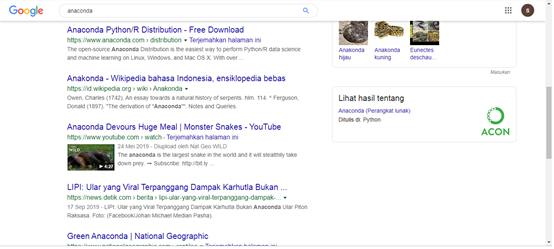
\includegraphics[scale=0.9]{gambar/1.png}
\caption{gambar1}
\label{fig:my_label}
\end{figure}[]

Selanjutnya klik download pada pojok kanan atas
\begin{figure}[h]
\centering
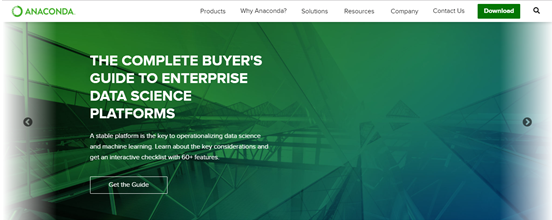
\includegraphics[scale=0.7]{gambar/2.png}
\caption{gambar2}
\label{fig:my_label}
\end{figure}[]

Kemudian pilih versi tergantung berapa bit laptop anda, kalau laptop anda 32 bit maka pakai yang 32 bit tapi jika laptop anda 64 bit maka pakailah yang 64 bit.
\begin{figure}[h]
\centering
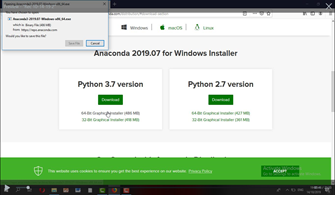
\includegraphics[scale=1.3]{gambar/3.png}
\caption{gambar3}
\label{fig:my_label}
\end{figure}

Selanjutnya klik I agree.
\begin{figure}[h]
\centering
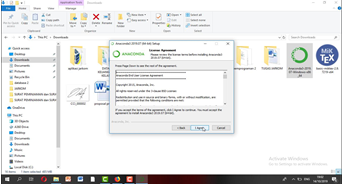
\includegraphics[scale=0.9]{gambar/4.png}
\caption{gambar4}
\label{fig:my_label}
\end{figure}

Lalu klik next
\begin{figure}[h]
\centering
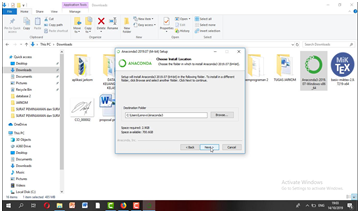
\includegraphics[scale=0.9]{section/5.png}
\caption{gambar5}
\label{fig:my_label}
\end{figure}

Kemudian akan mucul kotak dialog dan centang kedua-duanya, lalu klik install.
\begin{figure}[h]
\centering
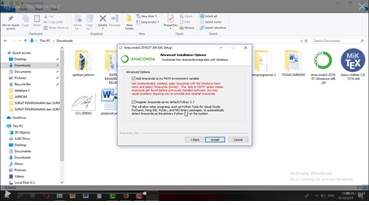
\includegraphics[scale=0.9]{section/6.png}
\caption{gambar6}
\label{fig:my_label}
\end{figure}

Tunggu hingga proses install selesai
\begin{figure}[h]
\centering
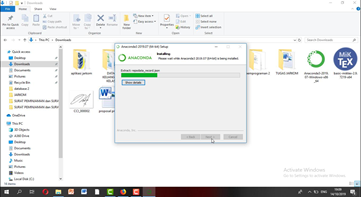
\includegraphics[scale=0.9]{section/7.png}
\caption{gambar7}
\label{fig:my_label}
\end{figure}

Setelah itu klik next
\begin{figure}[h]
\centering
    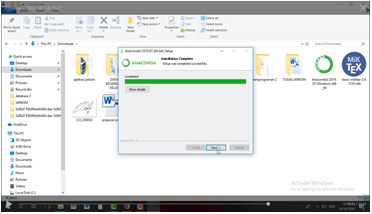
\includegraphics[scale=0.9]{section/8.png}
\caption{gambar9}
\label{fig:my_label}
\end{figure}

Kemudian klik next lagi
\begin{figure}[h]
\centering
    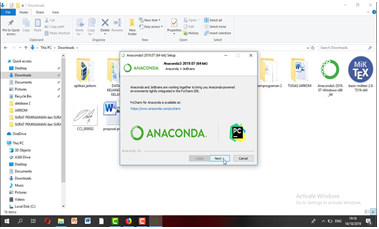
\includegraphics[scale=0.9]{section/9.png}
\caption{gambar9}
\label{fig:my_label}
\end{figure}


\begin{figure}[h]
\centering
    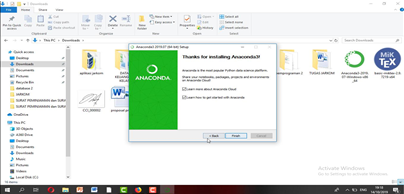
\includegraphics[scale=0.9]{section/10.png}
\caption{gambar10}
\label{fig:my_label}
\end{figure}


\section{CARA INSTALLER PIP}
Caranya agak mirip dengan install python, yaitu pertama searching pip pada google.
\begin{figure}[h]
\centering
    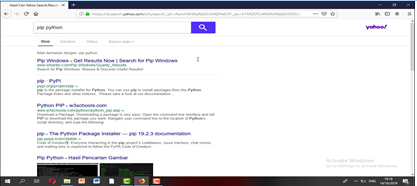
\includegraphics[scale=0.9]{section/41.png}
\caption{gambar11}
\label{fig:my_label}
\end{figure}

Lalu klik installation,seperti yang ditunjuk tanda panah.
\begin{figure}[h]
\centering
    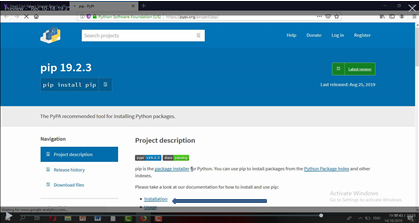
\includegraphics[scale=0.9]{section/42.png}
\caption{gambar12}
\label{fig:my_label}
\end{figure}

Kemudian klik get.pip.py seperti yang ditunjuk tanda panah dibawah ini, lalu klik ok.
\begin{figure}[h]
\centering
    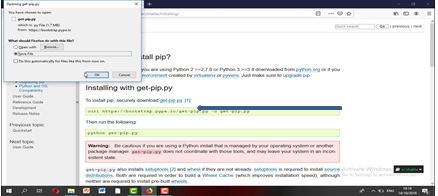
\includegraphics[scale=0.9]{section/43.png}
\caption{gambar13}
\label{fig:my_label}
\end{figure}

Setelah itu buka cmd
\begin{figure}[h]
\centering
    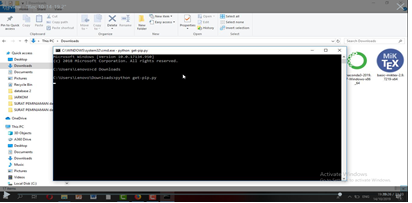
\includegraphics[scale=0.9]{section/44.png}
\caption{gambar14}
\label{fig:my_label}
\end{figure}

Lalu ketik  python get.pip.py
\begin{figure}[h]
\centering
    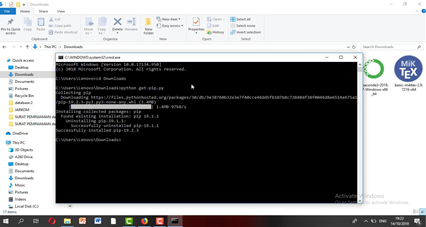
\includegraphics[scale=0.9]{section/45.png}
\caption{gambar15}
\label{fig:my_label}
\end{figure}

Jika tampilanya sudah seperti gambar yang dibawah ini, maka sudah selesai.
\begin{figure}[h]
\centering
    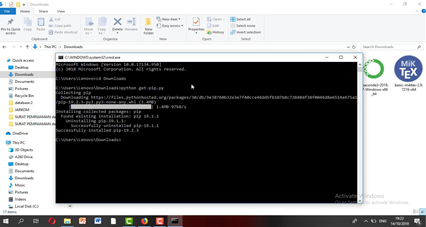
\includegraphics[scale=0.9]{section/45.png}
\caption{gambar16}
\label{fig:my_label}
\end{figure}

\section{CARA UPDATE SPYDER DAN ANACONDA}
Pertama buka aplikasi anacondanya
\begin{figure}[h]
\centering
    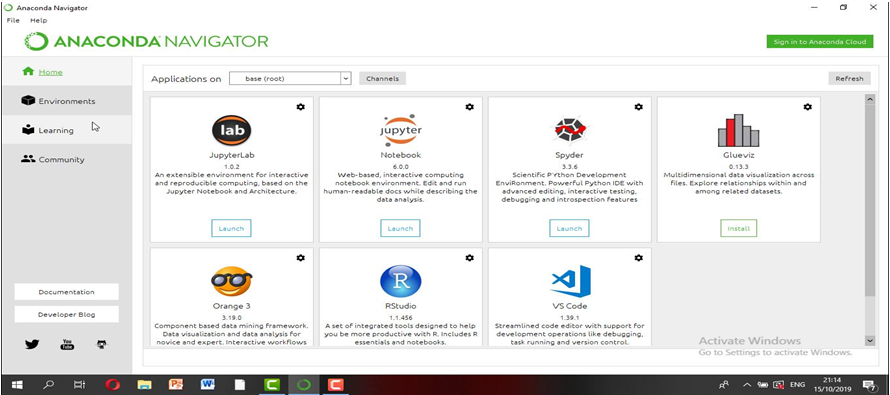
\includegraphics[scale=0.9]{section/51.png}
\caption{gambar17}
\label{fig:my_label}
\end{figure}

Setelah itu klik environments dan cari yang akan kita update
\begin{figure}[h]
\centering
    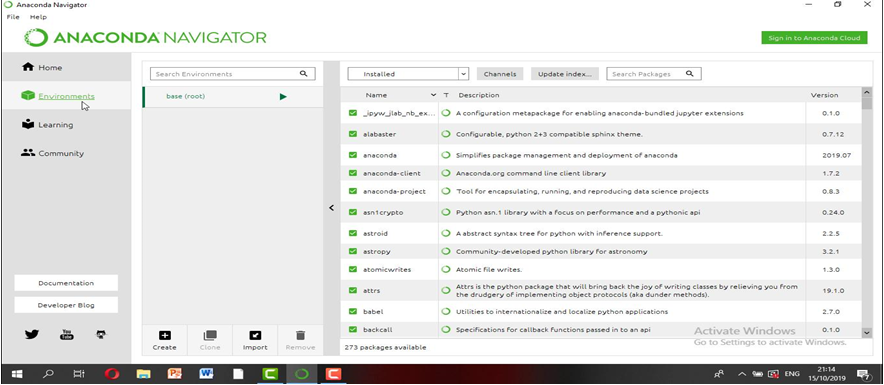
\includegraphics[scale=0.9]{section/52.png}
\caption{gambar18}
\label{fig:my_label}
\end{figure}

Lalu pilih spyder versi terbaru dari yang akan kita update
\begin{figure}[h]
\centering
    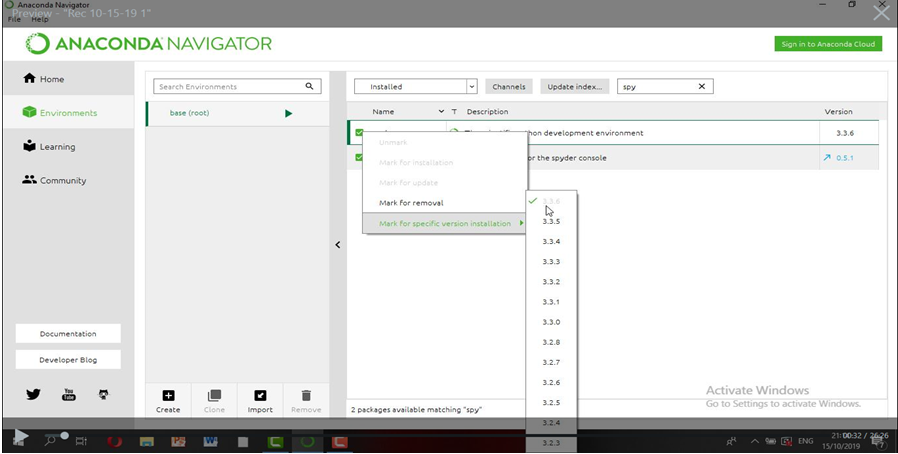
\includegraphics[scale=0.9]{section/53.png}
\caption{gambar19}
\label{fig:my_label}
\end{figure}

Begitu juga dengan anaconda yang akan kita update
\begin{figure}[h]
\centering
    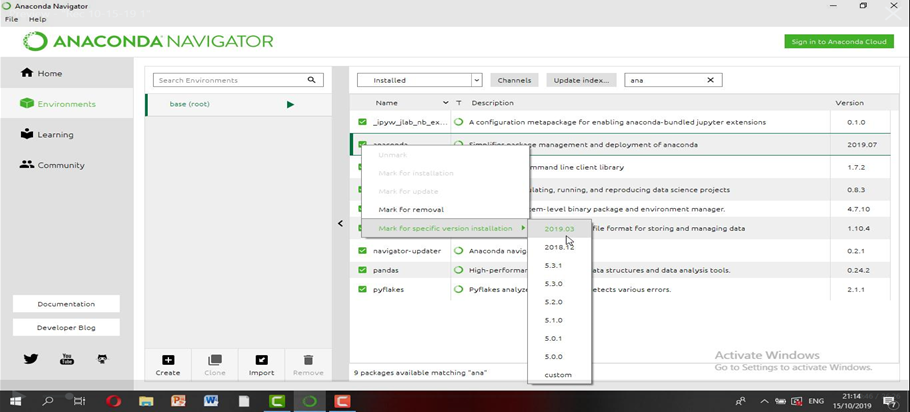
\includegraphics[scale=0.9]{section/54.png}
\caption{gambar20}
\label{fig:my_label}
\end{figure}

Setelah itu klik apply
\begin{figure}[h]
\centering
    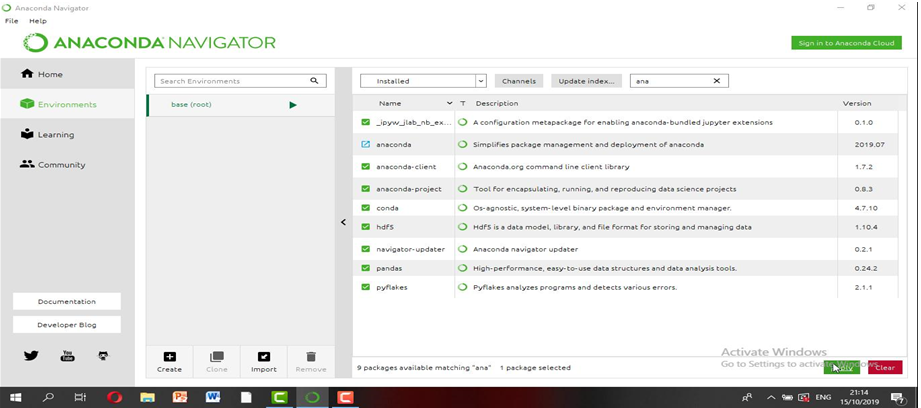
\includegraphics[scale=0.9]{section/55.png}
\caption{gambar21}
\label{fig:my_label}
\end{figure}

Dan tunggu sampai proses selesai
\begin{figure}[h]
\centering
    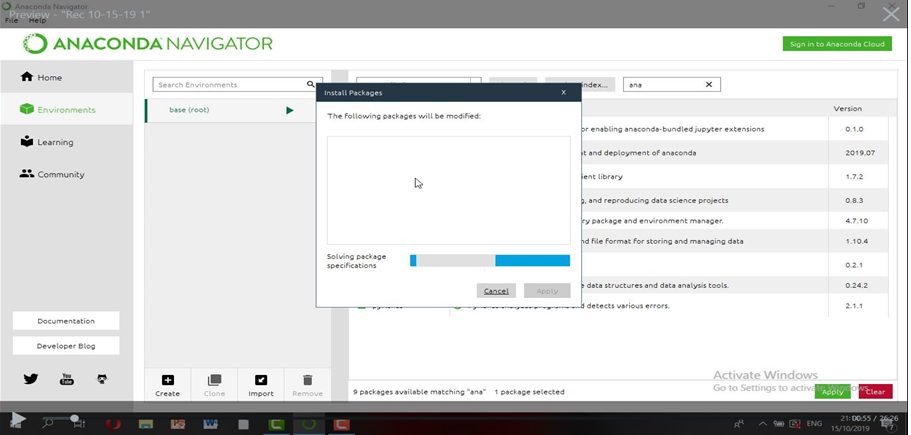
\includegraphics[scale=0.9]{section/56.png}
\caption{gambar22}
\label{fig:my_label}
\end{figure}

Jika sudah seperti tampilan dibawah ini, lalu klik apply lagi
\begin{figure}[h]
\centering
    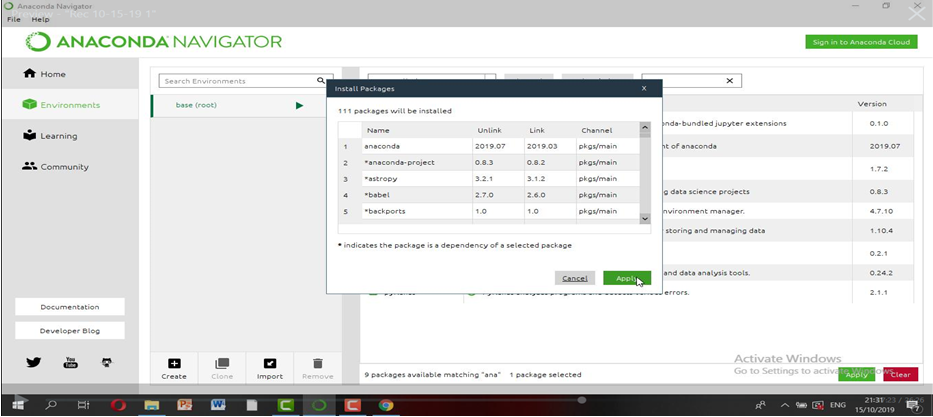
\includegraphics[scale=0.9]{section/57.png}
\caption{gambar23}
\label{fig:my_label}
\end{figure}

Kemudian tunggu sampai proses selesai
\begin{figure}[h]
\centering
    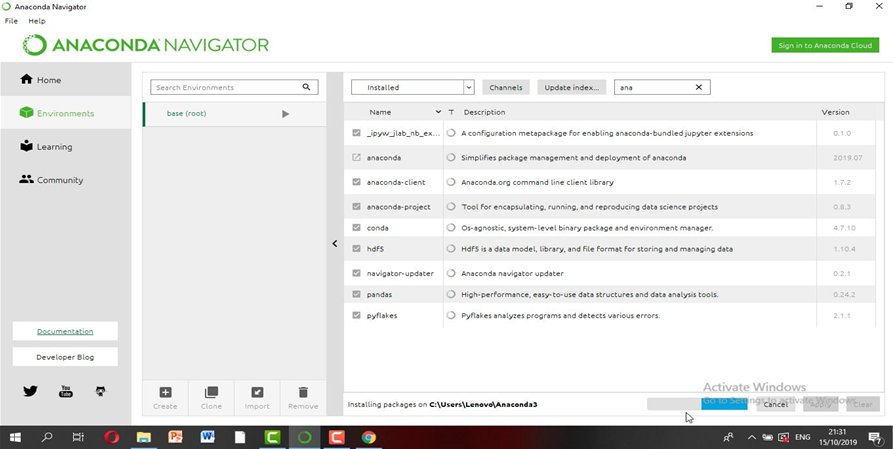
\includegraphics[scale=0.9]{section/58.png}
\caption{gambar24}
\label{fig:my_label}
\end{figure}

\section{Selenium}

from selenium.webdriver import Firefox
from selenium.webdriver.firefox.options import Options
from selenium.webdriver.common.desired_capabilities import DesiredCapabilities
from selenium.webdriver.firefox.firefox_binary import FirefoxBinary

print("Masukkan Npm Anda:")
npm = input()
print("Masukkan Password SIAP Anda:")
paswd = input('')

opsi = Options()

opsi.headless = False
binary = FirefoxBinary("C:\\Program Files\\Mozilla Firefox\\firefox.exe")
cap = DesiredCapabilities().FIREFOX
cap['marionette'] = True

browser=Firefox(executable_path='geckodriver.exe',
options=opsi,capabilities=cap,firefox_binary=binary)
browser.get('http://siap.poltekpos.ac.id/siap/besan.depan.php')

name = browser.find_element_by_name('user_name')
word = browser.find_element_by_name('user_pass')
login = browser.find_element_by_name('login')

name.send_keys(npm)
word.send_keys(paswd)
login.click(